\documentclass{article}

\textwidth=6.5in
\textheight=8.5in
\voffset=-54pt
\oddsidemargin=0in
\evensidemargin=0in
\setlength{\parskip}{8pt}
\setlength{\parindent}{0pt}

\usepackage{amsmath, amssymb}
\usepackage{ifthen}

\usepackage[inline]{enumitem}
\setlist{topsep=0pt, parsep=8pt}

\usepackage[rgb,table]{xcolor}\convertcolorsUfalse
\usepackage{graphicx}

% change hyperref options
\PassOptionsToPackage{hyphens}{url}
\usepackage[bookmarks,colorlinks,linkcolor=black,citecolor=blue,pdfstartview=FitH,urlcolor=blue]{hyperref}
\hypersetup{pdfpagemode=UseNone}
\usepackage{bookmark}

\usepackage{graphicx}
\usepackage{multicol}
\usepackage{framed}
\usepackage{array}

\usepackage{icomma}

\usepackage{marginnote}
\usepackage[colorinlistoftodos]{todonotes}
\renewcommand{\marginpar}{\marginnote}

\usepackage{soul}
\usepackage[normalem]{ulem}

\usepackage{pgfplots}
\pgfplotsset{compat=1.18}  
\pgfplotscreateplotcyclelist{mycolor}{black, blue, red, green!70!black, magenta, purple, cyan, orange }  
\pgfplotsset{
  disabledatascaling,
  cycle list=tikzcolor, 
  axis lines=middle,
  every axis plot/.style={no marks, thick},
  every axis/.style={
    enlarge x limits=false,
    enlarge y limits=auto,
    xlabel style={at={(current axis.right of origin)},anchor=west},
    ylabel style={at={(current axis.above origin)},anchor=south},
    % extra x and y ticks for asymptotes
    extra x tick style={grid=major, grid style={dashed,black}},
    extra y tick style={grid=major, grid style={dashed,black}},
    /pgf/number format/1000 sep={},
  },    
  tick label style = {font=\footnotesize, fill=\currentbgcolor, inner sep=0pt},    
  xticklabel shift=1pt,    
  scaled ticks=false,
  scaled y ticks=false,
  unbounded coords=jump,
  samples=101,
  minor tick length=0,
  scatter/classes={
    open={mark=*,draw=black,fill=white, mark size=2, thin},
    closed={mark=*,draw=black,fill=black, mark size=2, thin}
  },
  width=3in,
}
\pgfplotsset{open/.style={only marks, mark=*, fill=white, thin, mark size=2}}
\pgfplotsset{closed/.style={only marks, mark=*, draw=black, fill=black,
    thin, mark size=2}}
\pgfplotsset{labeled/.style={nodes near coords, only marks, mark=*, draw=black, fill=black, thin, mark size=2, point meta=explicit symbolic}}

\usepackage{tikz}
\usetikzlibrary{
  matrix,%
  % enables the snake paths
  decorations.pathmorphing,%
  % enables bigger arrows
  decorations.markings,%
  decorations.pathreplacing,%
  decorations.text,%
  calc,%
  patterns,%
  shapes.geometric,%
  arrows,
  decorations.shapes,
  positioning,
  plotmarks,
  intersections
}
\tikzset{>=latex} % sets default arrow type in tikz
\tikzset{font=\normalsize}
\tikzset{mark size=1.5pt, mark options=thin}
\tikzset{pin distance=4pt,
  every pin edge/.style={<-, thin, shorten <= -2pt}}

\interfootnotelinepenalty=10000
\renewcommand{\thefootnote}{(\arabic{footnote})}

\usepackage{multirow, bigdelim}

% change to \usepackage[sols]{handout} to see solutions
\usepackage[]{handout}

\newcommand\iscurrentenumi[1]{%
  \ifthenelse{\equal{#1}{\theenumi}}{}{#1}}
\setenumerate[1]{ref=\#\arabic*}
\setenumerate[2]{ref=\protect\iscurrentenumi{\theenumi}(\alph*)}
\newcommand\enumiiprefix[2]{%
  \ifthenelse{{\equal{#1}{\theenumi}}\AND{\equal{#2}{(\alph{enumii})}}}{}{}%
  \ifthenelse{{\equal{#1}{\theenumi}}\AND{\NOT{\equal{#2}{(\alph{enumii})}}}}{#2}{}%
  \ifthenelse{\equal{#1}{\theenumi}}{}{#1#2}%
}
\setenumerate[3]{ref=\protect\enumiiprefix{\theenumi}{(\alph{enumii})}\roman*}

\makeatletter

% underline links               
\let\@href=\href
\renewcommand{\href}[2]{\@href{#1}{\ul{#2}}}

\newcommand\calculator{
  
\begin{tikzpicture}[x=0.15ex, y=0.15ex, baseline=1.5pt]
    \begin{scope}[thick]
      \draw (0, 0) -- (10, 0) -- (10, 14) -- (0, 14) -- cycle;
      \foreach \x in {10/3, 20/3}
      {
        \draw (\x, 0) -- (\x, 10);
      }
      \foreach \y in {10/3, 20/3, 10}
      {
        \draw (0, \y) -- (10, \y);
      }
    \end{scope}
  \end{tikzpicture}
}
\newcommand{\calcitem}{\refstepcounter{enum\romannumeral\@enumdepth}%
\item[\calculator \csname labelenum\romannumeral\@enumdepth\endcsname]}

\makeatother

\definecolor{purple}{rgb}{0.5,0,1.0}
\definecolor{skyblue}{rgb}{0, 0.5, 1}

\newcommand{\highlight}[1]{\boldmath\hl{\textbf{#1}}\unboldmath}

\newcommand{\goal}[1]{\textbf{\textcolor{skyblue}{#1}}}

\newcommand{\doedfinity}[2][\newpage]{
  \begin{problem}[#1]
    Do the Edfinity assignment ``Problem Set #2''.

    We encourage you to write down any scratch work here, as well as
    things you want your future self to remember. Nothing you write
    here will be graded; it's just for you!
  \end{problem}
}

\newcommand{\psrnewpage}{\newpage}
\newcommand{\psreflection}[2][]{

  \ifthenelse{\not\equal{#1}{nocite}}{
    \begin{enumerate}[resume]
    \item
      \begin{problem}[1in]
        Please cite any help you got on this problem set:
        \begin{itemize}[nosep]
        \item If you worked with other students, please list their names here.
        \item If you used resources other than those on our Canvas site, please list them here.
        \end{itemize}
      \end{problem}

    \end{enumerate}
  }

  \probonly{%
    #2

    \psrnewpage

    \emph{Reflection space.} It's a good habit to take a few minutes at the end of each pset to reflect on what you learned and jot down notes to your future self. Here are a few reflection questions to get you started. Nothing you write here will be graded; it's just for you!
    \begin{itemize}
    \item Take a few minutes to look back at the problems. How could you explain to someone else how to do each problem? What was your strategy, and how did you know to use that strategy? If there are problems where you don't feel able to answer this, write down which ones they are. Come back to them in a few days when we post the homework solutions!

      \vspace{1.5in}

    \item Take a look back at the learning objectives on today's worksheet; how are you feeling about each one? If there are ones you know you need more practice with, write those down here.

      \vspace{1.5in}

    \item What did you find most challenging about this material? Do you have any lingering questions about it? If so, write them down here so you don't forget them. At some point, stop by office hours or MQC to ask!

      \vfill
    \end{itemize}      
  }
}

\usepackage{fancyhdr}
\lhead{\textcolor{white}{This content is protected and may not be shared, uploaded, or distributed.}}
\rhead{}
\rfoot{\vspace*{\fill}\footnotesize\textcopyright{} \emph{Harvard Math Ma}}
\renewcommand{\headrulewidth}{0pt}
\pagestyle{fancy}
\begin{document}

\begin{center}
  \large\textsc{Problem Set 25 - Derivatives of Exponential Functions}\vspace{.5in}\\
  \begin{problemonly}
   \large Name: \rule{5cm}{0.15mm}\\
   \end{problemonly}
\end{center}

\begin{enumerate}
\item  
  \note{
    \begin{itemize}[nosep]
    \item Some basic questions along the lines of: if $b$ is a number $> 1$ and you raise it to a really big positive power, what kind of result do you get? (Choices: very positive, positive but close to 0, etc.) 
    \item Basic derivatives, including one with a term $e^k$ to emphasize this is constant
    \item Match with graphs: $e^{ax}$ with $a > 0$, $e^{bx}$ with $b < 0$, $e^c$ with $c > 0$, $e^d$ with $d < 0$ (again to emphasize $e^c$ and $e^d$ are constants).
    \item Differentiate with Product Rule and Quotient Rule.
    \item Find a tangent line to $y = C e^x$
    \end{itemize}
  }

  \doedfinity{25}

\item Differentiate the following \uline{without} using the Quotient Rule. Show your work, and try to be efficient.

  \begin{enumerate}

  \item

    \begin{grading}
      2 points. They can also use the Product Rule instead of rewriting $g(t)$. 
    \end{grading}

    \begin{problem}[\vfill]
      $g(t) = e^t \left( e^{3t} + 2 \right) \left( e^{3t} - 2 \right)$
    \end{problem}

    \begin{solution}
      Let's rewrite $g(t)$ by distributing.
      \begin{align*}
        g(t) &= e^t(e^{3t}+2)(e^{3t}-2) \\
        &= e^t(e^{6t}-4) \\
        &= e^{7t} - 4e^t
      \end{align*}
      Now we can take the derivative using the rule that $\frac{d}{dx}e^{kx}= ke^{kx}$.
      \begin{align*}
        g'(t) &= \boxed{7e^{7t}-4e^t} 
      \end{align*}
    \end{solution}

  \item

    \begin{grading}
      2.5 points:
      \begin{itemize}[nosep]
      \item 0.5 for knowing $(xe^x)^7 = x^7 e^{7x}$
      \item 0.5 for knowing $\dfrac{e^{7x}}{e^{9x}} = e^{-2x}$
      \item 0.5 for recognizing the 2 in the denominator can be rewritten as multiplying by $\frac{1}{2}$
      \item 1 for differentiating correctly
      \end{itemize}
    \end{grading}

    \begin{problem}[\vfill]
      $\displaystyle h(x) = \frac{\left( x e^x \right)^7}{2e^{9x}}$
    \end{problem}

    \begin{solution}
      Let's rewrite $h(x)$ using exponent rules.
      \begin{align*}
        h(x) &= \frac{\left( x e^x \right)^7}{2e^{9x}} \\
        &= \frac{x^7e^{7x}}{2e^{9x}} \\
        &= \tfrac{1}{2}x^2e^{-2x}
      \end{align*}
      Now we can use the Product Rule.
      \begin{align*}
        h'(x) &= \frac{d}{dx} \tfrac{1}{2}x^2e^{-2x} \\
        &= \tfrac{1}{2} \left[(\tfrac{d}{dx}x^2)(e^{-2x})+(x^2)(\tfrac{d}{dx}e^{-2x})\right]\\
        &= \boxed{\tfrac{1}{2} \left[(2x)(e^{-2x})+(x^2)(-2e^{-2x})\right]}\\
        &= e^{-2x}(x-x^2)
      \end{align*}
    \end{solution}

  \end{enumerate}

\item \label{estimate-e}

  \begin{enumerate}
  \item \label{def-of-e}

    \begin{grading}
      1 point
    \end{grading}

    \begin{problem}[\vfill]
      In class, how did we define the number $e$? 
    \end{problem}

    \begin{solution} % Jason Bland
      We defined $e$ to be the number with the property that the line tangent to the graph of $y = e^x$ at $x = 0$ had slope 1. 
    \end{solution}

  \item \label{e-between-2-and-3}

    \begin{grading}
      1 point
    \end{grading}

    \begin{problem}[\vfill\newpage]
      Explain how we determined that $e$ must be between 2 and 3. 
    \end{problem}

    \begin{solution} % Jason Bland
      In class, we saw that the slope of $y = 2^x$ at $x = 0$ is less than 1 and the slope of $y = 3^x$ at $x = 0$ is greater than 1. The slope of $y = b^x$ at $x = 0$ increases with $b$, and the slope is 1 when $b = e$, so we must have $2 < e < 3$.
    \end{solution}

  \item
    Here's a way to get a better idea of how big $e$ is.  
    \begin{enumerate}
    \item

      \begin{grading}
        5 points:
        \begin{itemize}[nosep]
        \item 1 for knowing they need to find the tangent line at $x = 0$
        \item 2 for finding that tangent line correctly 
        \item 1 for plugging $x = 0.001$ into the tangent line to get the estimate
        \item 1 for explaining why it's an underestimate 
        \end{itemize}
      \end{grading}

      \begin{problem}[\vfill]
        Use linear approximation to estimate $e^{0.001}$. (Your answer should be a decimal that you can calculate by hand.) Is your estimate an overestimate or underestimate? Explain how you know.
      \end{problem}

      \begin{solution} 
        We'll find the tangent line to the graph of $f(x) = e^x$ at $x = 0$. Since $f'(x) = e^x$, this tangent line has slope $f'(0) = 1$. A point on the line is $(0, 1)$, so the equation of the tangent line is $y - 1 = 1 (x - 0)$, or $y = x + 1$. Therefore,
        \[ e^x \approx x + 1 \text{ for $x$ near 0}.\] Plugging in $x = 0.001$, $\boxed{e^{0.001} \approx 1.001}$. Since the graph of $e^x$ is always concave up, this is an \fbox{underestimate}.
      \end{solution}

    \calcitem

      \begin{grading}
        0.5 points
      \end{grading}

      \begin{problem}[\stretch{0.5}]
        Since $(e^{0.001})^{1000} = e$, raising your estimate for $e^{0.001}$ to the 1000th power will give you an estimate for $e$. Use a calculator or \href{https://www.wolframalpha.com}{WolframAlpha} to find this estimate.
      \end{problem}

      \begin{solution} % Jason Bland
        $e$ is roughly equal to (and slightly larger than) $1.001^{1000}
        \approx 2.71692$.
      \end{solution}

    \end{enumerate}

    \probonly{\emph{In fact, $e$ to 5 decimal places is $e \approx 2.71828$.}} 
  \end{enumerate}

  \pspace{\newpage}

\item %({\it 10.3.1})
  Let $\displaystyle f(x) = \frac{e^x}{x^2+1}$.

  \begin{enumerate}
  \item

    \begin{grading}
      1 point
    \end{grading}

    \begin{problem}[0.75in]
      What's the domain of $f$?
    \end{problem}

    \begin{solution}
      The domain of this function is \fbox{$(-\infty,\infty)$}, because there is no $x$ value for which the funtion is undefined.
    \end{solution}

  \item \label{e^x/(x^2+1)-critical-points}

    \begin{grading}
      4 points: 1 for correct derivative, 1 for finding the correct critical point, 2 for correctly classifying.

      The Second Derivative Test is inconclusive here; if students correctly calculate $f''(1) = 0$ and conclude it's neither a local minimum or local maximum, deduct 1. 
    \end{grading}

    \begin{problem}[\vfill]
      Find all critical points of $f$, and classify each as a local minimum, local maximum, or neither. Make sure to clearly communicate your justification; use words to let the reader know how you're classifying each critical point.
    \end{problem}

    \begin{solution}
      $$f(x)=\displaystyle \frac{e^x}{x^2+1}$$ $$f'(x)=\displaystyle \frac{(x^2)e^x-e^x(2x)}{(x^2+1)^2}=\displaystyle \frac{e^x(x^2-2x+1)}{(x^2+1)^2}=\displaystyle \frac{e^x(x-1)^2}{(x^2+1)^2}$$ So we have a critical point at \fbox{$x=1$}, since $f'(1)=0$. Plugging in values to the left and to the right of $x=1$ yields positive $f'(x)$ values, so this critical point is \fbox{neither a local maximum or minimum}.

      Note that the derivative can also be taken using the Chain Rule by first rewriting the function $f(x) = e^x(x^2+1)^{-1}$
      $$f'(x) = e^x(x^2+1)^{-1}+e^x(-(x^2+1)^{-2}(2x))=\frac{e^x}{x^2+1}-\frac{2xe^x}{(x^2+1)^2}=\frac{e^x(x^2+1)-2xe^x}{(x^2+1)^2}$$
      Once this is assembled over a common denominator, we have the same function as in the work with $f'(x)$ above. 
    \end{solution}

  \item

    \begin{grading}
      1.5 points. They can either use the fact that it's increasing everywhere on $[-2, 2]$, or they can plug the critical point and endpoints into $f$ to see which gives the highest value. 
    \end{grading}

    \begin{problem}[\nstretch{0.5}]
      Does $f$ have a global maximum on $[-2, 2]$? If so, where (at what $x$-value) does it occur, and how do you know? If not, why not?      
    \end{problem}

    \begin{solution}
      The Extreme Value Theorem guarantees that $f$ will have a global maximum on $[-2, 2]$.
      Since $f$ is always increasing, the maximum has to occur at $x=2$.
    \end{solution}

  \item

    \begin{grading}
      1.5 points
    \end{grading}

    \begin{problem}[\stretch{0.5}]
      Does $f$ have a global maximum on $(-\infty, \infty)$? If so, where (at what $x$-value) does it occur, and how do you know? If not, why not?
    \end{problem}

    \begin{solution}
      There is no global maximum on $(-\infty, \infty)$. Global extrema can only occur
      at critical points or at endpoints, and since the only critical point $x=1$ is
      neither a min nor a max, there are no global extrema on $(-\infty, \infty)$.
    \end{solution}

  \item

    \begin{grading}
      1 point
    \end{grading}

    \begin{problem}[1in]
      Find $\displaystyle \lim_{x \to -\infty} f(x)$. 
    \end{problem}

    \begin{solution}
      As $x \to -\infty$, the dominant term in the denominator is $x^2$.
      \begin{align*}
        \lim_{x \to -\infty} f(x) &= \lim_{x \to -\infty} \frac{e^x}{x^2+1} \\
        &= \lim_{x \to -\infty} \frac{e^x}{x^2} \\
        \intertext{As $x$ goes to $-\infty$, $e^x$ approaches zero and $x^2$ increases
        without bound, so}
        \lim_{x \to -\infty} f(x) &= \boxed{0}.
      \end{align*}
    \end{solution}

  \item

    \begin{grading}
      4 points:
      \begin{itemize}[nosep]
      \item 1 point for having a horizontal tangent line at each critical point they found in \ref{e^x/(x^2+1)-critical-points}
      \item 1 point for the increasing / decreasing behavior matching whatever they found in in \ref{e^x/(x^2+1)-critical-points}
      \item 1 point for being consistent with their $\displaystyle \lim_{x \to -\infty} f(x)$
      \item 1 point for the concavity matching the sign given sign chart
      \end{itemize}
    \end{grading}

    \begin{problem}[\vfill\newpage]
      Here's a sign chart for $f''$.
      \begin{center}
        \begin{tikzpicture}
          \begin{axis}[axis y line=none, x axis line style={-}, xtick={-0.179509, 1.}, xticklabels={$\approx -0.18$, $1$}, ymin=-2, height=1in, width=3in, clip=false]
            \addplot+[domain=-2.53853:2.17951, very thin]{0};
            \draw (-2.53853, -1.5) node[right] {sign of $f''$};
            \draw (-0.769264, -1.5) node{$+$};%
            \draw (0.410245, -1.5) node{$-$};%
            \draw (1.58975, -1.5) node{$+$};%
          \end{axis}
        \end{tikzpicture}
      \end{center}
      Use this, together with everything you've figured out in this problem, to sketch a graph of $f$. Make sure it's consistent with everything you've found. 
    \end{problem}

    \begin{solution}
      Based on the sign chart given for $f''(x)$, we know that $f$ is concave up on
      approximately $(-\infty, -0.18)$, concave down on $(-0.18, 1)$, and concave
      up on $(1, \infty)$. We also know that $f$ is always increasing, and
      that there is a horizontal tangent at $x=1$. Additionally, we know that
      $\lim_{x \to -\infty} f(x) = 0$, and that the $y$-intercept is $1$. 
      \begin{center}
        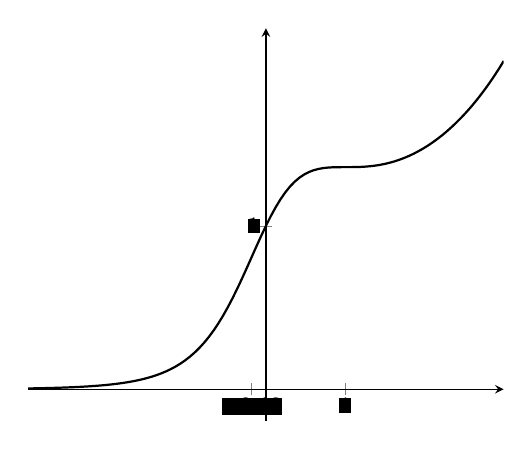
\begin{tikzpicture}
          \begin{axis}[ytick={1}, xtick={-0.18, 1}]
            \addplot[domain=-3:3] {(e^x)/(x^2+1)};
          \end{axis}
        \end{tikzpicture}
      \end{center}
    \end{solution}

  \end{enumerate}

\item % 10.3.20 modified 

  \begin{grading}
    10 points:
    \begin{itemize}[nosep]
    \item 1 for stating the goal
    \item 1 for having a correct formula for the perimeter in terms of $x$ and $y$
    \item 3 for correctly using the fact that the area of matting is 176 to get the perimeter in terms of one variable
    \item 2 for correctly finding the critical point of their perimeter function
    \item 2 for justifying that the critical point is a global min. They can use the First Derivative Test, Second Derivative Test, or end behavior. If they use the FDT or SDT, technically they should say there's only one critical point. Otherwise, they've only shown it's a local max / min, not a global one. If they omit this, please give them feedback and deduct 0.01 (just so they know there's some feedback). 
    \item 1 for answering the question (that is, giving the dimensions of the frame) 
    \end{itemize}
  \end{grading}

  \begin{problem}[\newpage]
    An artist wants to frame an 8-inch by 10-inch painting with matting. (In the picture below, the white part is the painting and the gray part is the matting. There is no matting under the painting.) She wants to use a total of 176 square inches of matting material, with $x$ inches of matting above and below the painting and $y$ inches of matting to the left and right of the painting.

    The frame, which goes around the outer edge of the matting, is expensive, so the artist wants to minimize the perimeter of the frame. What dimensions should the artist make the frame? 

    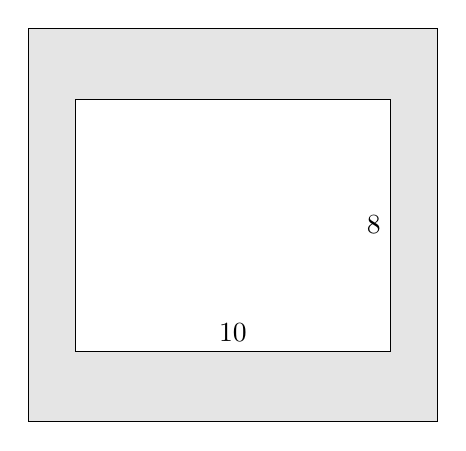
\begin{tikzpicture}[x=0.4cm, y=0.4cm]
      \filldraw[draw=black, fill=black!10!white] (-1.5, -2.25) -- (11.5, -2.25) -- (11.5, 10.25) -- (-1.5, 10.25) -- (-1.5, -2.25); % 
      \filldraw[draw=black, fill=white] (0, 0) -- node[above]{10} (10, 0) -- node[left] {8} (10, 8) -- (0, 8) -- (0, 0); %
    \end{tikzpicture}
  \end{problem}

  \begin{solution}
    \highlight{Goal:} Minimize the \goal{perimeter} of the frame.

    \highlight{Define variables:} We'll use $P$ to represent the perimeter of the frame, 
    along with the variables given in the problem, $x$, which is the length of matting
    above or below the painting, and $y$, the length of the matting to the left or right.

    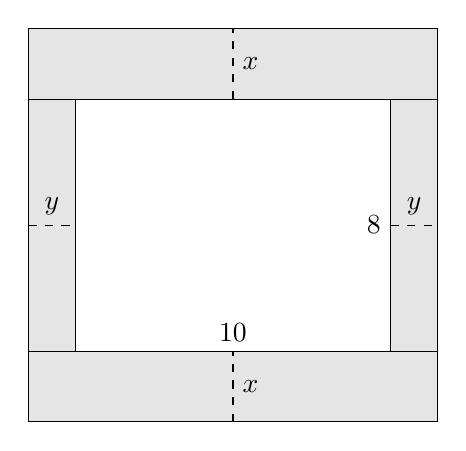
\begin{tikzpicture}[x=0.4cm, y=0.4cm]
      \filldraw[draw=black, fill=black!10!white] (-1.5, -2.25) -- (11.5, -2.25) -- (11.5, 10.25) -- (-1.5, 10.25) -- (-1.5, -2.25); % 
      \filldraw[draw=black, fill=white] (0, 0) -- node[above]{10} (10, 0) -- node[left] {8} (10, 8) -- (0, 8) -- (0, 0); %
      \draw[dashed] (5, -2.25) -- node[midway, right] {$x$} (5, 0);
      \draw[dashed] (5, 8) -- node[midway, right] {$x$} (5, 10.25);
      \draw[dashed] (-1.5, 4) -- node[midway, above] {$y$} (0, 4);
      \draw[dashed] (10, 4) -- node[midway, above] {$y$} (11.5, 4);
      \draw (-1.5, 8) -- (0, 8);
      \draw (10, 8) -- (11.5, 8);
      \draw (-1.5, 0) -- (0, 0);
      \draw (10, 0) -- (11.5, 0);
    \end{tikzpicture}

    
    \highlight{Formula for goal:} Since the frame will go around the matting, the width will be $10+2y$ and the length will be $8+2x$. So, the perimeter is $P=2(10+2y+8+2x)=36+4y+4x$.

    Now we need to \highlight{relate the variables using information from the problem.} 
    We're told the area of the matting is $176$ square inches. We can write a formula
    for the area of the matting by dividing it up into four rectangles.
    \[
    176=2x(10+2y)+2y(8)=20x+4xy+16y,
    \] and we can solve for $y$ and get \[y=\frac{44-5x}{x+4}.\] Substituting
    this into our formula for the perimeter gives us 
    \[P(x)=36+4\left(\frac{44-5x}{x+4}\right)+4x.\]
    The minimum value of $x$ is $0$, and the maximum value corresponds to when $y=0$.
    Since $y=\frac{44-5x}{x+4}$, we can set this equal to $0$ to determine that when $y=0$,
    $x=\frac{44}{5}$. So the domain is $0 \leq x \leq \frac{44}{5}$.

    \highlight{Critical points:} We can find $P'(x)$ using the Quotient Rule. 
    \begin{align*}
      P'(x) &= \frac{d}{dx} \left[36+4\left(\frac{44-5x}{x+4}\right)+4x\right] \\
      &= \frac{d}{dx}36 + 4\frac{d}{dx}\!\left(\frac{44-5x}{x+4}\right) + \frac{d}{dx}4x \\
      &= 0+ 4\left(\frac{(\frac{d}{dx}(44-5x))(x+4)-(44-5x)(\frac{d}{dx}(x+4))}{(x+4)^2} 
      \right) + 4 \\
      &= 4\left(\frac{(-5)(x+4)-(44-5x)(1)}{(x+4)^2}\right) + 4 \\
      &= 4\left(\frac{-64}{(x+4)^2}\right) +4 \\
      &= \frac{-256}{(x+4)^2} + 4 \\
    \end{align*} 
    Note that the derivative of the middle term can also be found using the Chain Rule (we will differentiate only that term below):
    \begin{align*}
        \frac{d}{dx}\!\left(\frac{44-5x}{x+4}\right) &=\frac{d}{dx}\!\left((44-5x)(x+4)^{-1}\right)\\
        &=(-5)(x+4)^{-1}+(44-5x)(-(x+4)^{-2} (1))\\
        &=\dfrac{-5}{x+4}-\dfrac{44-5x}{(x+4)^2}\\
        &= \dfrac{-5(x+4)}{(x+4)^2}-\dfrac{44-5x}{(x+4)^2}\\
        &=\dfrac{-5x-20-44+5x}{(x+4)^2}\\
        &=\dfrac{-64}{(x+4)^2}
    \end{align*}
    $P'(x)$ is undefined when $x=-4$, but this isn't in the domain. Setting $P'(x)$ equal
    to zero and solving:
    \begin{align*}
      \frac{-256}{(x+4)^2} + 4 &= 0 \\
      \frac{256}{(x+4)^2} &= 4 \\
      (x+4)^2 &= 64 \\
      x+4 &= \pm 8 \\
      x= 4 &\text{ or } x=-12
    \end{align*}
    The only critical point within the domain is $x=4$.

    \highlight{Global minimum:} Since there's only one critical point on the domain,
    if we can show it's a local min, then it's the global min. Let's use the First Derivative
    Test. Testing values around $x=4$ gives us the following sign chart.
      \begin{center}
        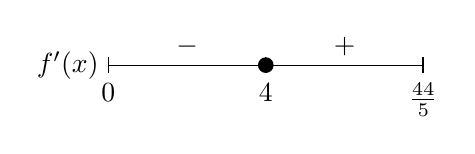
\begin{tikzpicture}
          \draw[|-|] (-2,0) -- (2, 0);
          \node[left] at (-2,0) {$f'(x)$};
          \draw[shift={(0,0)},color=black] (0pt,3pt) -- (0pt,-3pt) node[below] {$4$};
          \draw[shift={(-2,0)},color=black] (0pt,3pt) -- (0pt,-3pt) node[below] {$0$};
          \draw[shift={(2,0)},color=black] (0pt,3pt) -- (0pt,-3pt) node[below] 
          {$\frac{44}{5}$};
          \node[circle, fill=black, inner sep=2pt] at (0,0) {};
          \node[above] at (-1,0) {$-$};
          \node[above] at (1,0) {$+$};
        \end{tikzpicture}
      \end{center}
      This shows that there is a local min at $x=4$ which is also the global min.
    
     \highlight{Answer the question:} Finally, we find our $y$ dimension: $y=\frac{44-5(4)}
     {4+4}=\frac{24}{8}=3$. Therefore to minimize the cost, the artist should make the frame
     \fbox{16 inches wide and 16 inches tall}.
  \end{solution}

\end{enumerate}
\psreflection{For next class, read \href{https://canvas.harvard.edu/files/20608906/download?download_frd=1}{\S 4.2 of \emph{Functions Modeling Change} by Connally et. al} through Example 1.}
\end{document}
